% BEGIN SECTION 1 - MILAN
% Last updated by Milan Ilnyckyj 2013-06-24


		\singlespacing
		\section{Executive summary}
		\label{sec:ExecutiveSummary}
		\doublespacing



The governments of the world, including the government of Canada, have agreed we should avoid raising global temperatures to more than 2˚C above where they were before we started burning fossil fuels.\footcite[][]{CopenhagenAccord}
This is the threshold at which the world has agreed that climate change becomes ``dangerous''.
Based on hundreds of thousands of years of evidence on how the climate responds to greenhouse gases (GHGs), we can calculate that avoiding a 2˚C increase means we must keep future GHG pollution to no more than 565 billion tonnes (gigatonnes) of carbon dioxide (\ce{CO2}).\footcite[For an excellent summary that is accessible to non-experts see: ][]{TerrifyingNewMath}
At the same time, we know that burning the world's proven reserves of coal, oil, and natural gas would produce 2,795 gigatonnes of \ce{CO2} --- nearly five times as much as it would be safe to burn.\footcite[][]{CTI2012} \footcite[Another accessible summary of the issue can be found in: ][]{HotBackyard}



Climate change is a defining example of social injury.
Firms that produce fossil fuels do not bear any economic burden as a result of the many forms of harm they are imposing on other people, including agricultural impacts, sea level rise, human health impacts, and more severe extreme weather.
Likewise, those who use fossil fuels enjoy the benefits while imposing these costs on others.
In order to avoid severe global injury, the total quantity of fossil fuels burned by humanity must be capped at a level far below the level of fossil fuels available to be burned. As \emph{The Economist} explains: ``[C]ompanies and governments already have far more oil, gas and coal than they need... assuming temperatures are not to rise by more than 2˚C''.\footcite[][]{EconomistUnburnable}
The business plans of fossil fuel companies do not take this reality into account.
They assume they can burn all of their proven reserves, along with any additional reserves they discover in unconventional areas like the arctic, the deep ocean, and Canada's bituminous sands.
Right now, we are adding about 30 gigatonnes (billions of tonnes) of \ce{CO2} to the atmosphere each year, and the amount we add is increasing at a rate of about 3\%.
That means that we are on track to exceed the 565 gigatonne limit within 15 years.



Two implications arise from this. 
First, we need to find a way to meet the world's energy needs while leaving 80\% of the world's fossil fuel reserves unburned.\footnote{For a detailed rebuttal of the argument that carbon capture and storage eliminates this necessity, see: \nameref{CCSSaves}.} 
As NASA climatologist James Hansen explains: ``Rapid reduction of fossil fuel emissions is required for humanity to
succeed in preserving a planet resembling the one on which civilization developed''.\footcite[][]{HansenPaleo}
This requires a massive redirection of investment from fossil fuel energy sources to different energy sources that do not alter the climate.
Second, the stockmarket value of fossil fuel companies is based on the outdated assumption that fossil fuel extraction and use can continue without limit.
If this occurs, the global effects will be catastrophic.
As such, much of the value of these companies is illusory, based on an out-dated assumption that we can use the atmosphere forever as a free dumping ground for \ce{CO2}.


Figure \ref{fig:TwoDegreeBudget} from the Carbon Tracker Initiative summarizes the situation the world now finds itself in, with regard to fossil fuels.
On the left are two circles depicting the total `carbon budget' the world can make use of without breaching the 2˚C barrier, with the black circle showing what has already been burned and the grey circle showing what could still be burned without breaking the budget limit.
The circles to the right depict the massive quantity of potential \ce{CO2} emissions embedded in the world's remaining coal, oil, and gas.\footcite[][p. 6]{CTI2012}



\begin{figure}
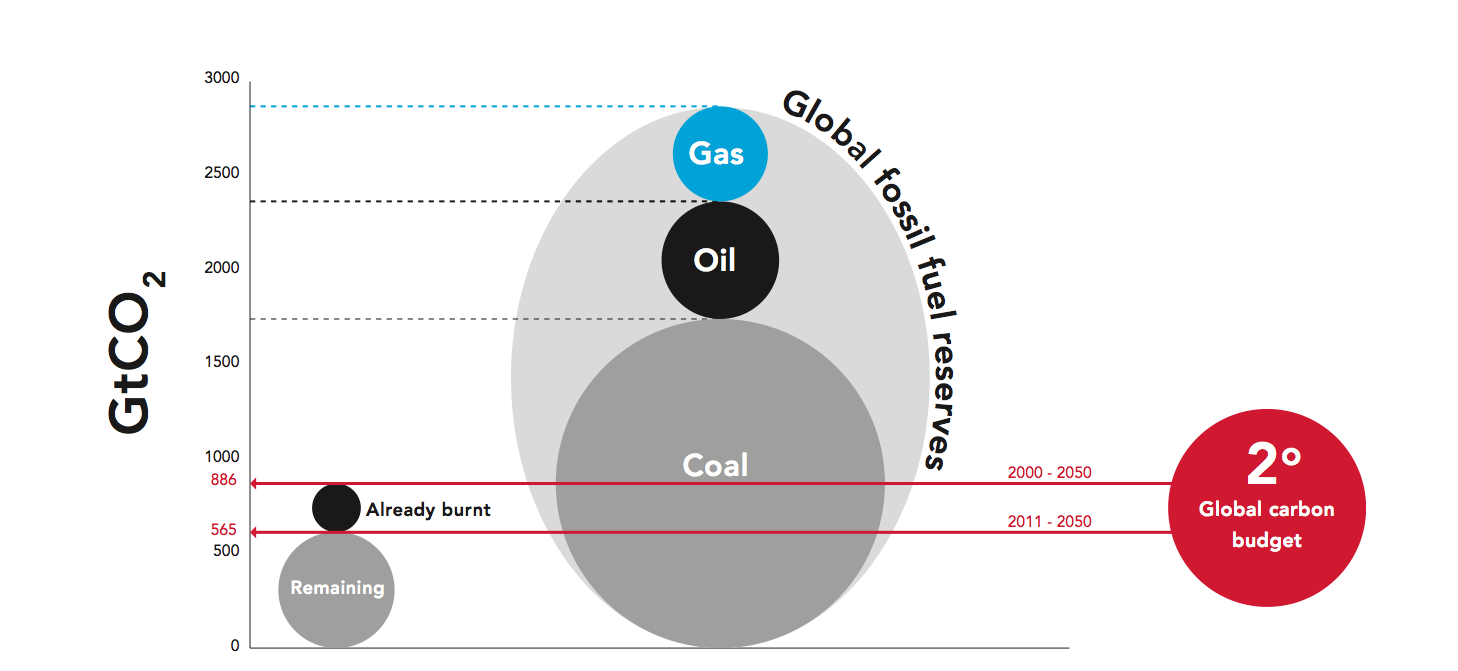
\includegraphics[width=\textwidth]{s1-carbon-budget.png}
\centering
\caption{Comparison of the global 2˚C carbon budget with fossil fuel reserves \ce{CO2} emissions potential}
\label{fig:TwoDegreeBudget}
\end{figure}




\textbf{How the University of Toronto can make a difference}



The International Energy Agency expects \$37 trillion to be spent on energy supply infrastructure between 2012 and 2035.\footcite[][]{IEA2012factsheet}
Humanity must decide whether to spend this money digging ourselves deeper into a pit of fossil fuel dependence, or whether to redirect it toward moving beyond fossil fuels.
The University of Toronto can take part in the redirection of investment that is necessary to prevent climatic catastrophe by selling its shares in fossil fuel companies before investors at large accept that most of their reserves are unburnable.
To avoid dangerous climate change, the whole world must progressively replace its fossil-fuel-intensive energy infrastructure with one that is compatible with climate stability.
This requires the massive redirection of investment away from new fossil fuel facilities like pipelines and unconventional oil and gas facilities and toward cost-effective approaches to \ce{CO2} mitigation, including energy conservation and renewable energy deployment.\footcite[The consultancy McKinsey \& Company has studied and ranked global mitigation options, in terms of their cost, plausible deployment speed, and their capacity to mitigate greenhouse gas pollution. See: ][p. 8]{McKinseyCurve}



Universities, which collectively have endowments and pension funds worth many billions of dollars, can play an important role in driving this shift.
University divestment of fossil fuel company shares would demonstrate that the `smart money' is sufficiently concerned about climate change to take meaningful action, and could prompt other investors to reconsider their own investment decisions. 
Divestment would help decrease investor confidence in the viability of new projects like coal-fired power plants and oil pipelines, while maintaining an overall portfolio with stable ands attractive returns.



The authors and supporters of this brief therefore call upon the University of Toronto to:
\begin{itemize}
	\item Make an immediate statement of principle, expressing its intention to divest its direct holdings of stock in fossil fuel companies within five years,
	\item Immediately stop making new investments in the industry,
	\item Instruct its investment managers to wind down the university’s existing direct stock holdings in the 200 fossil fuel companies listed in \nameref{sec:200Companies} over five years, and
	\item Divest from Royal Dutch Shell by the end of 2013.
\end{itemize}



Divestment from Royal Dutch Shell should be a high priority for the University of Toronto. 
In addition to being a major contributor to climate change, Shell has an ongoing history of social injury, both in Canada and around the world. 
As the university's single largest international equity holding, Shell sends the message that the University of Toronto is committed to fossil fuel exploitation. 
Divestment would send the opposite message: that it is committed to addressing climate change.  
The university would not suffer financially as a consequence of divesting from Shell and, by doing so, it would protect itself from the risks created by this investment.



Across North America, the peer schools of the University of Toronto are considering divestment.
There include Harvard, Yale, Princeton, Stanford, and MIT.
[NUMBER] schools have already committed to divest.\footnote{For an up-to-date list, see: \url{http://gofossilfree.org/commitments/}}
By leading the way and becoming the first major university to divest, the University of Toronto can distinguish itself as being ahead of the pack on one of the major issues of the 21st century.



\begin{vcom}
Finalize the number of schools in the paragraph above when the rest of the brief is done.
\end{vcom}



The University of Toronto's Statement of Institutional Purpose includes ``a resolute commitment to the principles of equal opportunity, equity and justice.'' \footcite{InstitutionalPurpose}
If future generations are to have equal opportunities, they cannot inherit a planet that has been impoverished by uncontrolled climate change.
Similarly, the principles of equity and justice forbid us from ignoring what we know about the harms of greenhouse gas pollution by continuing to impose risk and suffering on innocent people around the world and in future generations.
Canada, Toronto, and the University of Toronto have historically benefitted from fossil fuel use far exceeding the global \emph{per capita} average.
Having benefited for decades from behaviour that we now know to be extremely damaging, the university has a special moral obligation to be part of the solution.



By choosing to divest, the University of Toronto can improve its financial prospects, uphold its values, and take part in a necessary global transition away from CO2-intensive forms of energy. 



% END SECTION 1 - MILAN